\documentclass[xcolor={usenames,dvipsnames,svgnames}, compress, aspectratio=169, 11pt]{beamer}

\usepackage{booktabs}
\usepackage{multirow}
\usepackage{dcolumn}
\usepackage{colortbl}
\usepackage{xcolor}
\usepackage{hyperref}
\usepackage{amsmath}
\usepackage{wrapfig}
\usepackage{algorithm}
\usepackage[noend]{algpseudocode} 
\usepackage{pifont}
\usepackage[style=authoryear-icomp,backend=bibtex, mincitenames=2, maxcitenames=2]{biblatex}
\usepackage{marvosym}
\usepackage{mathtools}
\usepackage{array}
\usepackage[export]{adjustbox}
\usepackage{bm}
\usepackage{dsfont}
\usepackage{subcaption}

\usepackage[font=scriptsize]{caption}

\newcommand{\argmax}{\operatornamewithlimits{argmax}}
\newcommand{\argmin}{\operatornamewithlimits{argmin}}
\newcommand{\nodeset}[1]{\bm{\mathsf{#1}}}
\newcommand{\cbar}{\,|\,}
\newcommand{\cndbar}{\,|\,}
\newcommand{\SPN}{\mathcal{S}}
\newcommand{\Node}{\mathsf{N}}
\newcommand{\Leaf}{\mathsf{L}}
%\newcommand{\Node}{\mathcal{N}}
\newcommand{\SumNode}{\mathsf{S}}
\newcommand{\ProdNode}{\mathsf{P}}
\newcommand{\DistNode}{\mathsf{D}}
\newcommand{\Nodes}{\bm{\mathsf{N}}}
\newcommand{\DistNodes}{\bm{\mathsf{D}}}
\newcommand{\SumNodes}{\bm{\mathsf{S}}}
\newcommand{\ProdNodes}{\bm{\mathsf{P}}}
\newcommand{\ch}{\mathsf{ch}}
\newcommand{\scope}{\mathsf{sc}}

\newcommand{\x}{\mathbf{x}}
\newcommand{\unaryminus}{\scalebox{0.75}[1.0]{\( - \)}}

\newcolumntype{R}[2]{
  >{\adjustbox{angle=#1,lap=\width-(#2)}\bgroup}
  l
  <{\egroup}
}

\newcommand*\rot{\multicolumn{1}{R{45}{1em}}}
\newcommand{\rbm}[2]{%
  \mathrel{\raisebox{#1}{$#2$}}%
}

\newcommand{\comment}[3][\small]{\begin{minipage}{1\linewidth}
          \raggedleft
          {
            $\color{violet}\boldsymbol\Rightarrow$
            #1
            {\emph{#2}}
          }
      \end{minipage}#3\\
}

\usetheme{spinaceto}

% %\addtobeamertemplate{footnote}{}{\vspace{16pt}}
% \newcommand{\customcite}[1]{\footnote{\tiny \citeauthor{#1},
%     \citetitle{#1}, \citeyear{#1}}}
% \newcommand{\customcitenomark}[1]{\footnotenomarkleft{\tiny
%     \citeauthor{#1}, \citetitle{#1}, \citeyear{#1}}}
% \newcommand{\customcitetext}[1]{\footnotenomarkleft{\tiny \citeauthor{#1}, \citetitle{#1}, \citeyear{#1}}}

\newcommand{\cmark}{\ding{51}}%
\newcommand{\xmark}{\ding{55}}

\setbeamersize{text margin left=8mm}

% \setbeamertemplate{bibliography item}{\hspace{10pt}\raise
%   .2ex\hbox{\textcolor{lacamlilac}{$\boldsymbol{\oplus}$}}}

\addbibresource{referomnia.bib}



\definecolor{wwine} {HTML} {cccaa9}
\definecolor{rwine} {HTML} {770a2d}
\definecolor{abagreen} {HTML} {2ca02c}
\definecolor{abapink} {HTML} {e377c2}
\definecolor{abagray} {HTML} {7f7f7f}
\definecolor{abayellow} {HTML} {bcbd22}
\definecolor{ababrown} {HTML} {8c564b}


\begin{document}

\title{\httm[.3]{mpigreen}{\emph{Automatic Bayesian}}\\[-5pt]
    \httm[.3]{mpigreen}{\emph{Density Analysis}}}
%\subtitle{\small \emph{or they joys and pains of exact inference}}
\author{
  \authorbox[90pt]{\emph{Antonio Vergari}}{Max-Plank-Institute IS}{\dag}\hspace{2pt}
    \authorbox[100pt]{Alejandro Molina}{TU Darmstadt}{\ddag}\hspace{-10pt}
    \authorbox[90pt]{Robert Peharz}{University of Cambridge}{\S}\\[5pt]
    \authorbox[100pt]{Zoubin Ghahramani}{University of Cambridge\\
      Uber AI Labs}{\S}\hspace{-8pt}
    \authorbox[100pt]{Kristian Kersting}{TU Darmstadt}{\ddag}\hspace{-10pt}
    \authorbox[90pt]{Isabel Valera}{Max-Plank-Institute IS}{\dag}\\
    % \vspace{15pt}
\includegraphics[width=20pt]{figures/logo1}
  }
\date{31st January 2019 - \textbf{AAAI19 \emph{Honolulu}}}
% \institute{Department of Computer Science, University of Bari ``Aldo Moro'', Bari, Italy
% \and 
% Department of Physics, University of Bari ``Aldo Moro'', Bari, Italy
% \and
% National Institute for Nuclear Physics (INFN), Bari Division, Bari, Italy
% }

% \institute{\textbf{Max-Planck-Institute}
%       \par \textbf{for Intelligent Systems}}
% \department{Probabilistic Learning}
\institutelogo{figures/mpi-minerva}
\institutesize{30pt}

% \secondinstitute{\textbf{TU Darmstadt}}
% \seconddepartment{Computer Science\\Department}
\secondinstitutelogo{figures/tu-darmstadt-athena.png}
\secondinstitutesize{25pt}

% \thirdinstitute{\textbf{University of} \\\textbf{Cambridge}}
% \thirddepartment{Engineering Department}
\thirdinstitutelogo{figures/cam-logo-big.png}
\thirdinstitutesize{25pt}


% \lablogo{\includegraphics[height=25pt]{figures/cam-logo-big-gray}}
% \otherlogo{\includegraphics[height=35pt]{figures/darms}}
% \otherlaboratory{TU Darmstadt}
% \othergroup{Computer Science Department}

\makeatletter
% \addtobeamertemplate{headline}{\vspace{-30pt}}{\hspace{10pt}}
% \defbeamertemplate*{frametitle}{custom-spinaceto}[1][]
% {
%   \vskip15pt%
%   \insertframetitle\par
%   \ifdefined\insertframesubtitle
%   \usebeamerfont{framesubtitle}\insertframesubtitle
%   \fi
% }
% \makeatother


{
  \setbeamertemplate{headline}{}
  \setbeamertemplate{footline}{}
  \begin{frame}
    \titlepage
  \end{frame}
}


% \begin{frame}[t, htt=mpigreen]
%   \frametitle{In a nutshell}

%   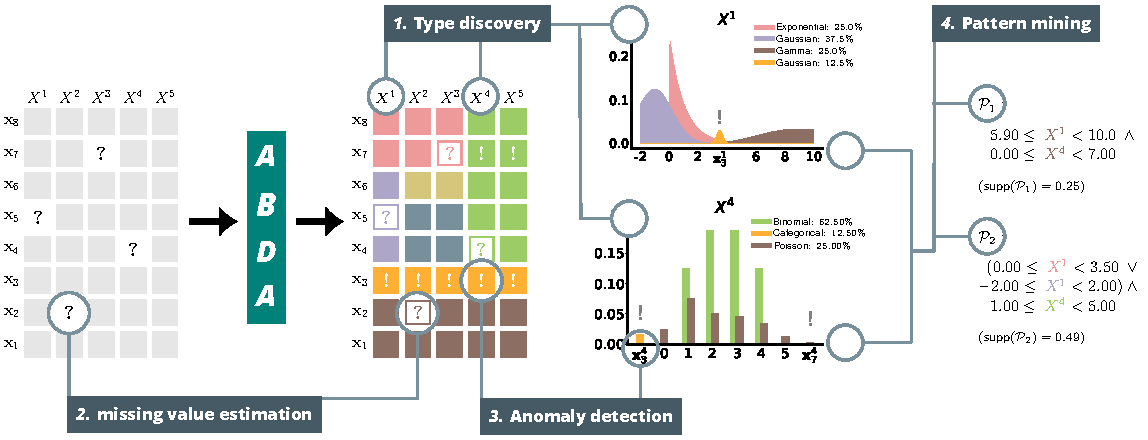
\includegraphics[width=1.04\linewidth]{figures/abda-full}
  
% \end{frame}



\begin{frame}[t, htt=bgrey2]
  \frametitle{Exploratory data analysis}
  
\end{frame}

\begin{frame}[t, htt=bgrey2]
  \frametitle{Real world data}

  \large
  \begin{minipage}[t]{0.6\linewidth}
    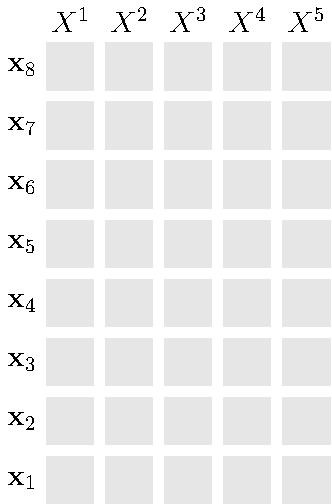
\includegraphics[width=.4\linewidth]{figures/abda-grid-empty}
  \end{minipage}\hfill\begin{minipage}[t]{0.3\linewidth}
    \vspace{-150pt}
    Real world data is\par
  \end{minipage}  
\end{frame}


\begin{frame}[t, htt=bgrey2]
  \frametitle{Real world data}

  \large
  \begin{minipage}[t]{0.6\linewidth}
    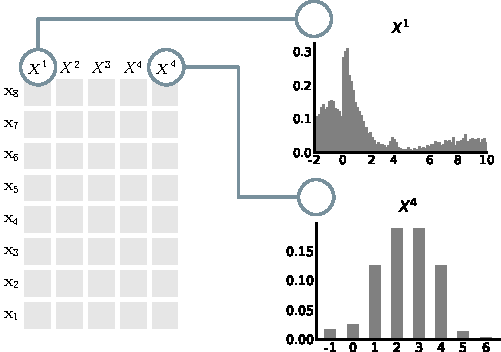
\includegraphics[width=.99\linewidth]{figures/abda-hist-type}
  \end{minipage}\hfill\begin{minipage}[t]{0.3\linewidth}
    \vspace{-150pt}
    { Real world data is}\\[5pt]
    \htt[lacamlilac]{\textbf{\emph{heterogeneous}}}\\
    \comment[\normalsize]{mixed discrete and continuous RVs}{}\\
    \comment[\normalsize]{mixed likelihood models}{}\\
    % \htt[lacamlilac]{\textbf{\emph{incomplete}}}\\
    % \htt[lacamlilac]{\textbf{\emph{anomalous}}}\\
  \end{minipage}  
\end{frame}

\begin{frame}[t, htt=bgrey2]
  \frametitle{Real world data}

  \large
  \begin{minipage}[t]{0.6\linewidth}
    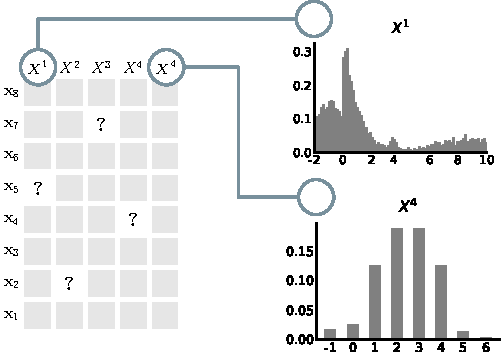
\includegraphics[width=.99\linewidth]{figures/abda-miss-hist-type}
  \end{minipage}\hfill\begin{minipage}[t]{0.3\linewidth}
    \vspace{-150pt}
    { Real world data is}\\[5pt]
    \htt[lacamlilac]{\textbf{\emph{heterogeneous}}}\\
    % \comment[\normalsize]{mixed discrete and continuous RVs}{}\\
    % \comment[\normalsize]{mixed likelihood models}{}\\
    \htt[lacamlilac]{\textbf{\emph{incomplete}}}\\
    \comment[\normalsize]{missing values}{}\\
    %\htt[lacamlilac]{\textbf{\emph{anomalous}}}\\
  \end{minipage}  
\end{frame}


\begin{frame}[t, htt=bgrey2]
  \frametitle{Real world data}

  \large
  \begin{minipage}[t]{0.6\linewidth}
    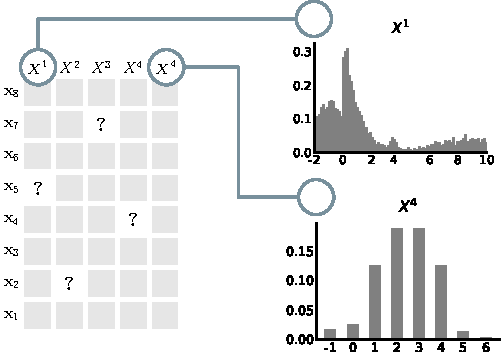
\includegraphics[width=.99\linewidth]{figures/abda-miss-hist-type}
  \end{minipage}\hfill\begin{minipage}[t]{0.3\linewidth}
    \vspace{-150pt}
    { Real world data is}\\[5pt]
    \htt[lacamlilac]{\textbf{\emph{heterogeneous}}}\\
    % \comment[\normalsize]{mixed discrete and continuous RVs}{}\\
    % \comment[\normalsize]{mixed likelihood models}{}\\
    \htt[lacamlilac]{\textbf{\emph{incomplete}}}\\
    % \textbf{potentially}
    % \htt[lacamlilac]{\textbf{\emph{spourious}}}\\
    \htt[lacamlilac]{\textbf{\emph{dirty}}}\\
    \comment[\normalsize]{containing anomalies: novelties, outliers, etc\dots}{}\\
  \end{minipage}  
\end{frame}


\begin{frame}[t, htt=bgrey2]
  \frametitle{Real world data}

  \large
  \begin{minipage}[t]{0.6\linewidth}
    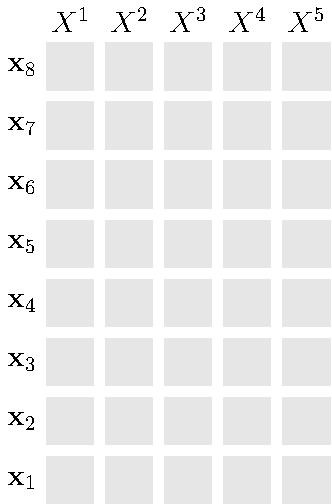
\includegraphics[width=.4\linewidth]{figures/abda-grid-empty}
  \end{minipage}\hfill\begin{minipage}[t]{0.3\linewidth}
    \vspace{0pt}
    Real world data is\par
  \end{minipage}  
\end{frame}


\begin{frame}[t, htt=bgrey2]
  \frametitle{Exploratory data analysis}

  \large
  \begin{minipage}[t]{0.6\linewidth}
    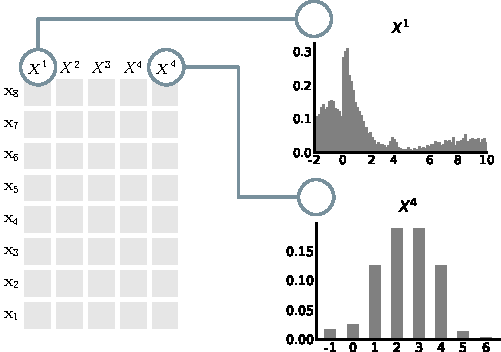
\includegraphics[width=.99\linewidth]{figures/abda-hist-type}
  \end{minipage}\hfill\begin{minipage}[t]{0.4\linewidth}
    \vspace{-150pt}
    {The ``data understanding'' pipeline}\\[5pt]
    \htt[lacamlilac]{\textbf{\emph{infer statistical types}}}\\
    \comment[\normalsize]{is it a positive continuous RV?}{}\\
    \comment[\normalsize]{is it an ordinal RV?}{}\\
    % \htt[lacamlilac]{\textbf{\emph{incomplete}}}\\
    % \htt[lacamlilac]{\textbf{\emph{anomalous}}}\\
  \end{minipage}  
\end{frame}

\begin{frame}[t, htt=bgrey2]
  \frametitle{Exploratory data analysis}

  \large
  \begin{minipage}[t]{0.6\linewidth}
    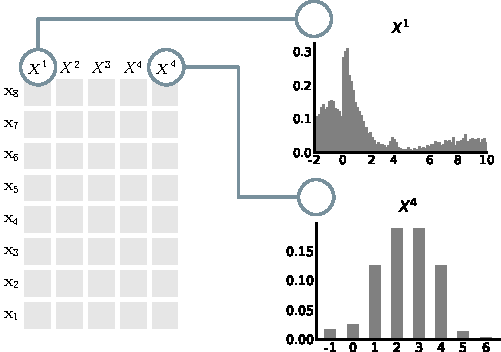
\includegraphics[width=.99\linewidth]{figures/abda-hist-type}
  \end{minipage}\hfill\begin{minipage}[t]{0.4\linewidth}
    \vspace{-150pt}
    {The ``data understanding'' pipeline}\\[5pt]
    \htt[lacamlilac]{\textbf{\emph{infer statistical types}}}\\
    \htt[lacamlilac]{\textbf{\emph{infer likelihood models}}}\\
    \comment[\normalsize]{is it Gaussian?}{}\\
    \comment[\normalsize]{is it Poisson?}{}\\
    % \htt[lacamlilac]{\textbf{\emph{incomplete}}}\\
    % \htt[lacamlilac]{\textbf{\emph{anomalous}}}\\
  \end{minipage}  
\end{frame}


\begin{frame}[t, htt=bgrey2]
  \frametitle{Exploratory data analysis}

  \large
  \begin{minipage}[t]{0.6\linewidth}
    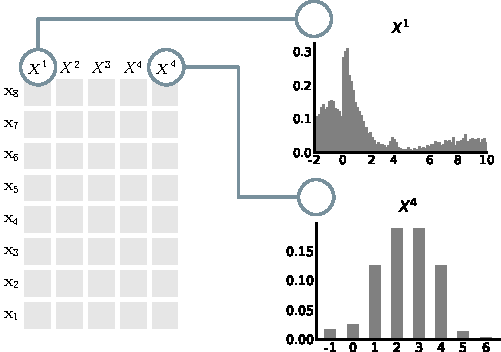
\includegraphics[width=.99\linewidth]{figures/abda-hist-type}
  \end{minipage}\hfill\begin{minipage}[t]{0.4\linewidth}
    \vspace{-150pt}
    {The ``data understanding'' pipeline}\\[5pt]
    \htt[lacamlilac]{\textbf{\emph{infer statistical types}}}\\
    \htt[lacamlilac]{\textbf{\emph{infer likelihood models}}}\\
    \htt[lacamlilac]{\textbf{\emph{infer dependency structure}}} among
    RVs\\
    \comment[\normalsize]{does $X^{4}$ depend on $X^{1}$?}{}\\
    \comment[\normalsize]{structure learning}{}\\
    % \htt[lacamlilac]{\textbf{\emph{anomalous}}}\\
  \end{minipage}  
\end{frame}


\begin{frame}[t, htt=bgrey2]
  \frametitle{Exploratory data analysis}

  \large
  \begin{minipage}[t]{0.6\linewidth}
    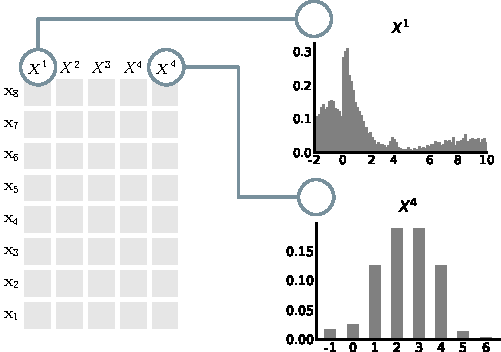
\includegraphics[width=.99\linewidth]{figures/abda-hist-type}
  \end{minipage}\hfill\begin{minipage}[t]{0.4\linewidth}
    \vspace{-150pt}
    {The ``data understanding'' pipeline}\\[5pt]
    \htt[lacamlilac]{\textbf{\emph{infer statistical types}}}\\
    \htt[lacamlilac]{\textbf{\emph{infer likelihood models}}}\\
    \htt[lacamlilac]{\textbf{\emph{infer dependency structure}}} among
    RVs\\
    \htt[lacamlilac]{\textbf{\emph{missing value estimation}}}\\
  \end{minipage}  
\end{frame}


\begin{frame}[t, htt=bgrey2]
  \frametitle{Exploratory data analysis}

  \large
  \begin{minipage}[t]{0.6\linewidth}
    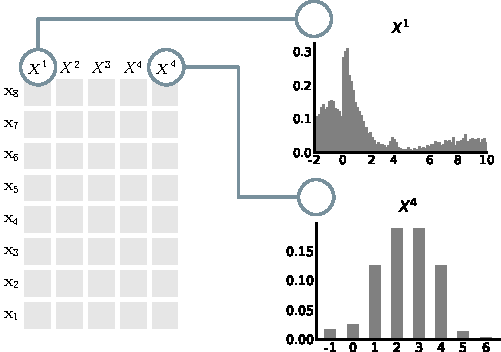
\includegraphics[width=.99\linewidth]{figures/abda-hist-type}
  \end{minipage}\hfill\begin{minipage}[t]{0.4\linewidth}
    \vspace{-150pt}
    {The ``data understanding'' pipeline}\\[5pt]
    \htt[lacamlilac]{\textbf{\emph{infer statistical types}}}\\
    \htt[lacamlilac]{\textbf{\emph{infer likelihood models}}}\\
    \htt[lacamlilac]{\textbf{\emph{infer dependency structure}}} among
    RVs\\
    \htt[lacamlilac]{\textbf{\emph{missing value estimation}}}\\
    \htt[lacamlilac]{\textbf{\emph{anomaly detection}}}\\
  \end{minipage}  
\end{frame}


\begin{frame}[t, htt=mpigreen]
  \frametitle{Automatic exploratory data analysis for non-statisticians}

  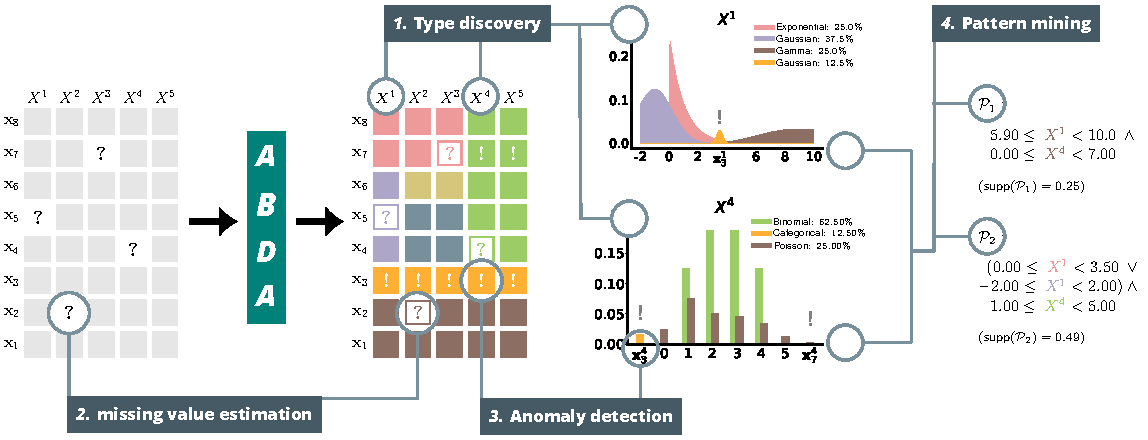
\includegraphics[width=1.04\linewidth]{figures/abda-full}\\

  with ABDA we automate exploratory data analysis and make it
  accessible for non-statisticians!
  
\end{frame}

\begin{frame}[t, htt=bgrey2]
  \frametitle{ABDA: representation}

  \large
  \begin{minipage}[t]{0.3\linewidth}
    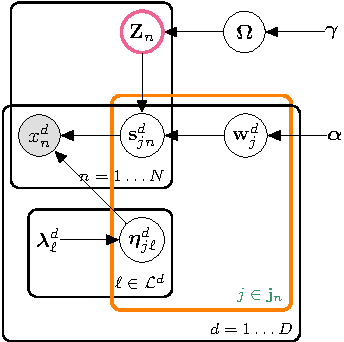
\includegraphics[width=.99\linewidth]{figures/joint-param-hspn-crop}
  \end{minipage}\hfill\begin{minipage}[t]{0.4\linewidth}
    \vspace{-150pt}
      ABDA captures  correlations among random variables RVs via
  \emph{\textbf{latent variables} (LVs)} at
  a \htt[pink2]{\textbf{\emph{top level}}} 
  while modeling heterogeneous distributions at a
  \htt[gold2]{\textbf{\emph{bottom level}}}
  
  \end{minipage}  
\end{frame}

\begin{frame}[t, htt=bgrey2]
  \frametitle{ABDA: representation}

  \large
  \begin{minipage}[t]{0.3\linewidth}
    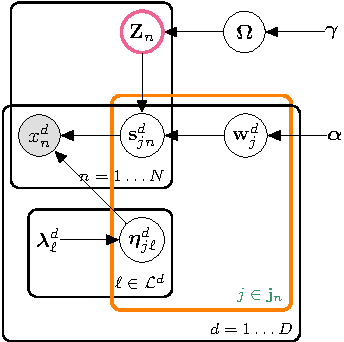
\includegraphics[width=.99\linewidth]{figures/joint-param-hspn-crop}
  \end{minipage}\hfill\begin{minipage}[t]{0.3\linewidth}
    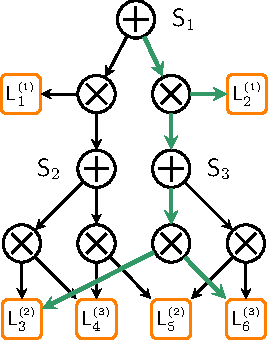
\includegraphics[width=.99\linewidth]{figures/hspn}
  \end{minipage}\hfill\begin{minipage}[t]{0.4\linewidth}
    \vspace{-150pt}
      capturing  correlations among random variables RVs via
  \emph{\textbf{latent variables} (LVs)} at
  a \htt[pink2]{\textbf{\emph{top level}}} via a \emph{\textbf{Sum-Product
    Network}} (\textbf{SPN})~\cite{Poon2011} 
  \end{minipage}  
\end{frame}

\begin{frame}[t, htt=bgrey2]
  \frametitle{ABDA: representation}

  \large
  \begin{minipage}[t]{0.3\linewidth}
    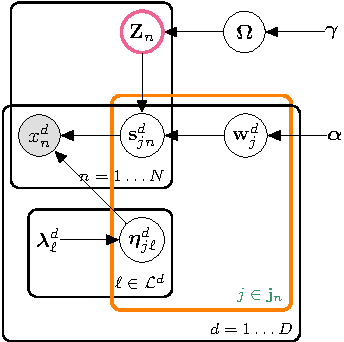
\includegraphics[width=.99\linewidth]{figures/joint-param-hspn-crop}
  \end{minipage}\hfill\begin{minipage}[t]{0.3\linewidth}
    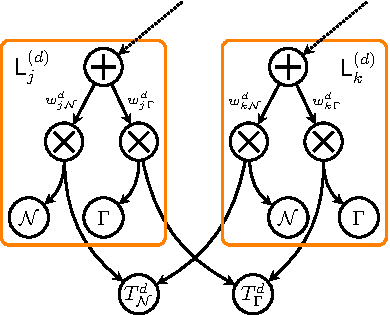
\includegraphics[width=.99\linewidth]{figures/type-leaf-crop}
  \end{minipage}\hfill\begin{minipage}[t]{0.4\linewidth}
    \vspace{-150pt}
      the 
  \htt[gold2]{\textbf{\emph{bottom level}}}
  via \textbf{\emph{dictionaries of likelihood models}} $\mathcal{L}^{d}$ for each
  feature $d$
  \end{minipage}  
\end{frame}


\begin{frame}[t, htt=bgrey2]
  \frametitle{SPNs}

  \large
  \begin{minipage}[t]{0.3\linewidth}
    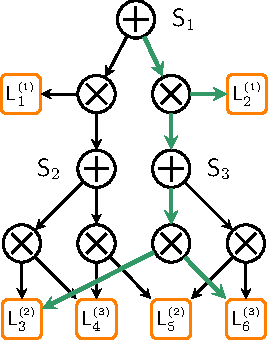
\includegraphics[width=.99\linewidth]{figures/hspn}
  \end{minipage}\hfill\begin{minipage}[t]{0.3\linewidth}
    \vspace{-150pt}
    sum nodes represents mixtures\\
    product nodes are factorizations over independent RVs\\
    leaf nodes are smaller tractable models
  \end{minipage}\hfill\begin{minipage}[t]{0.4\linewidth}
    \vspace{-150pt}
    inference is tractable in SPNs:\\
    to marginalize any RV\\
    to compute conditionals\\
    to perform MPE (approximate)\\
  \end{minipage}  
\end{frame}

\begin{frame}[t, htt=bgrey2]
  \frametitle{ABDA: learning and inference}

  \large
  \begin{minipage}[t]{0.6\linewidth}
    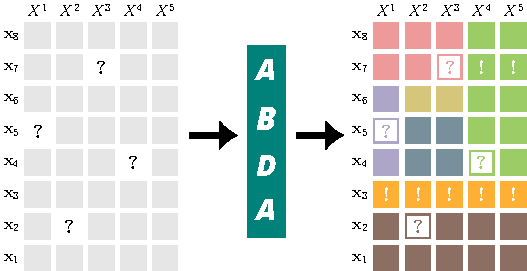
\includegraphics[width=.99\linewidth]{figures/abda-partitioning}
  \end{minipage}\hfill\begin{minipage}[t]{0.3\linewidth}
    \vspace{-150pt}
    data-agnostic structure learning\\

    partitioning of the data\\

    efficient inference via Gibbs sampling
    
  \end{minipage}  
\end{frame}

\begin{frame}[t, htt=bgrey2]
  \frametitle{Type inference}

  \large
  \begin{minipage}[t]{0.6\linewidth}
    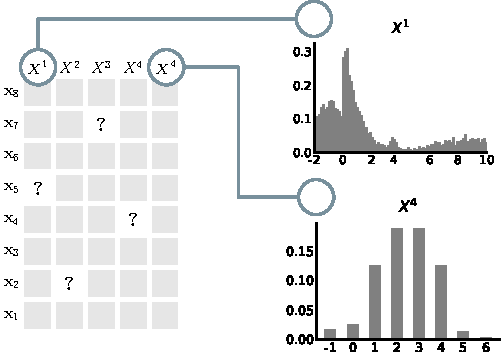
\includegraphics[width=.99\linewidth]{figures/abda-miss-hist-type}
  \end{minipage}\hfill\begin{minipage}[t]{0.3\linewidth}
    \vspace{-150pt}
    
    
  \end{minipage}  
\end{frame}

\begin{frame}[t, htt=bgrey2]
  \frametitle{Type inference}

  \large
  \begin{minipage}[t]{0.66\linewidth}
    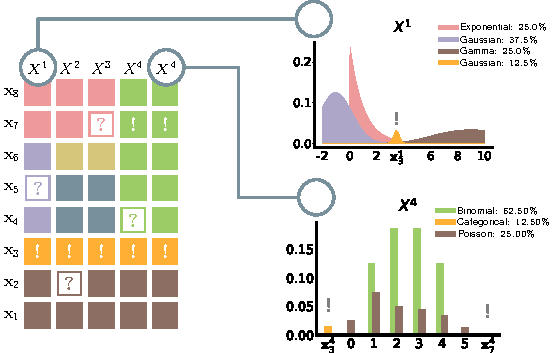
\includegraphics[width=.99\linewidth]{figures/abda-type-inf}
  \end{minipage}\hfill\begin{minipage}[t]{0.3\linewidth}
    \vspace{-150pt}
    Best likelihood models explaining the data are inferred from the
    dictionary via Gibbs sampling\\

    Mixture proportions represent uncertainty over likelihood models\\

    Therefore, one can reason about uncertainty over statistical types
    as well\\
    
  \end{minipage}  
\end{frame}

\begin{frame}[t, htt=bgrey2]
  \frametitle{Type inference}

  \large
  \begin{minipage}[t]{0.5\linewidth}
    %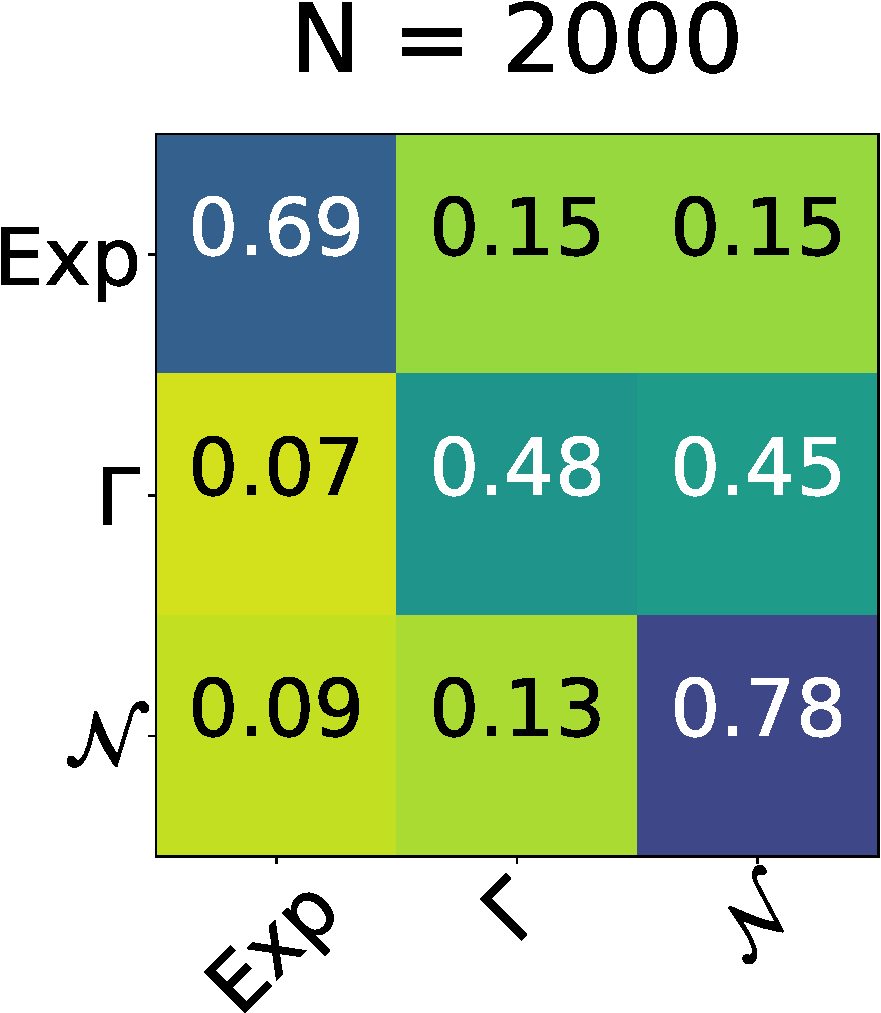
\includegraphics[width=.5\linewidth]{figures/N-2000-cont-param-conf-mat-crop}
    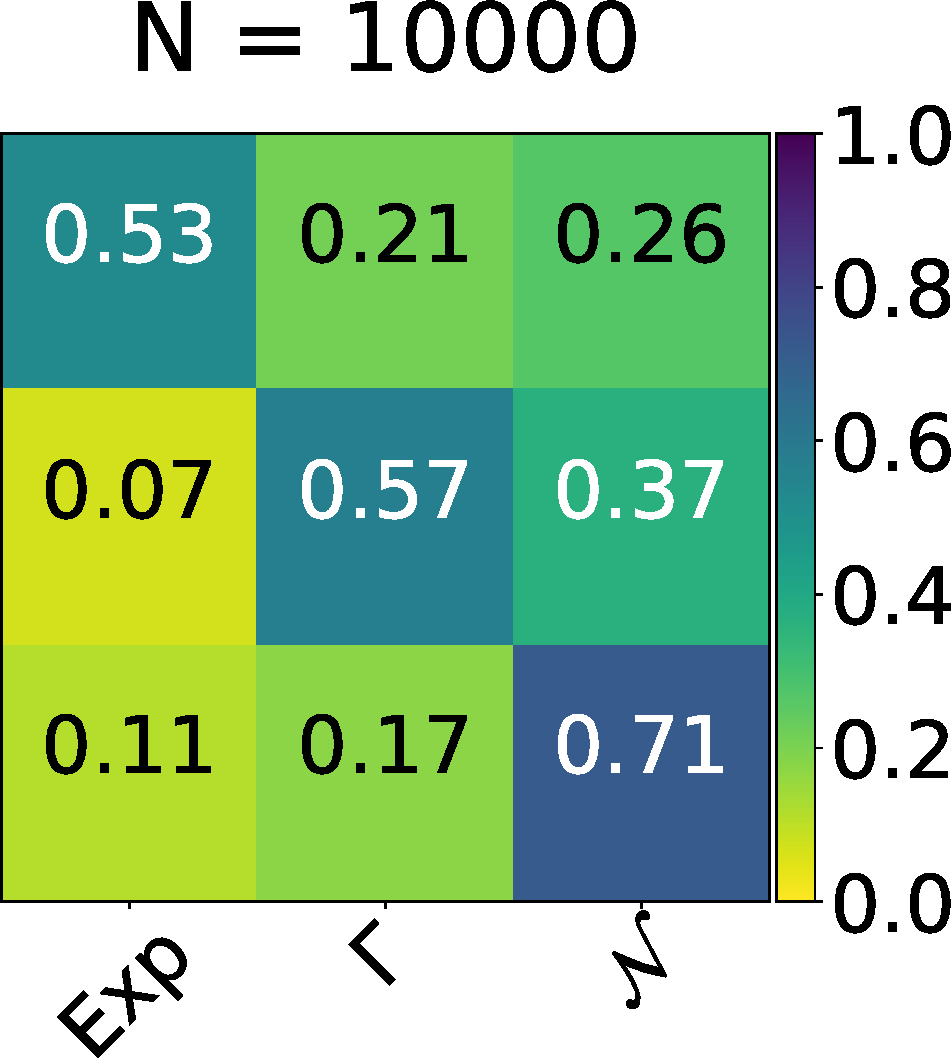
\includegraphics[width=.5\linewidth]{figures/N-10000-cont-param-conf-mat-crop}
    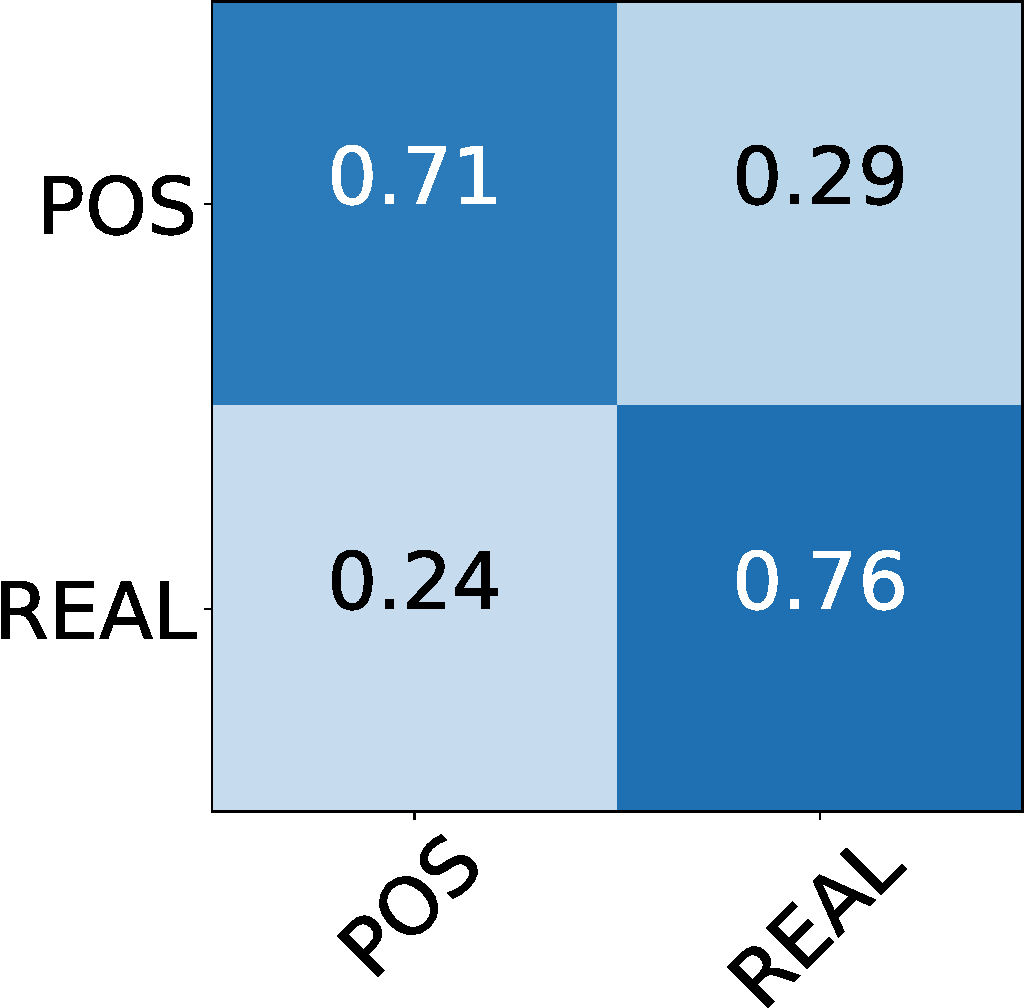
\includegraphics[width=.5\linewidth]{figures/cont-types-conf-mat-crop}\\
    %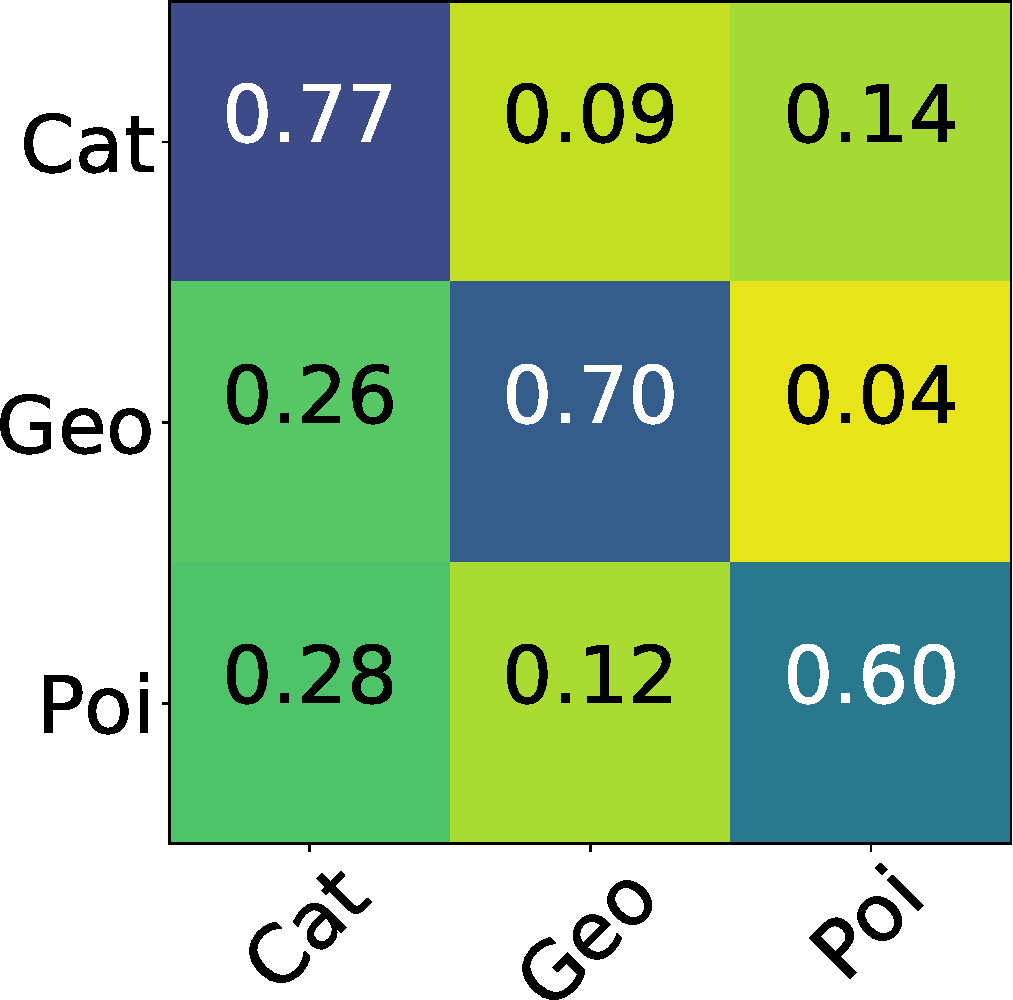
\includegraphics[width=.5\linewidth]{figures/N-2000-disc-param-conf-mat-crop}
    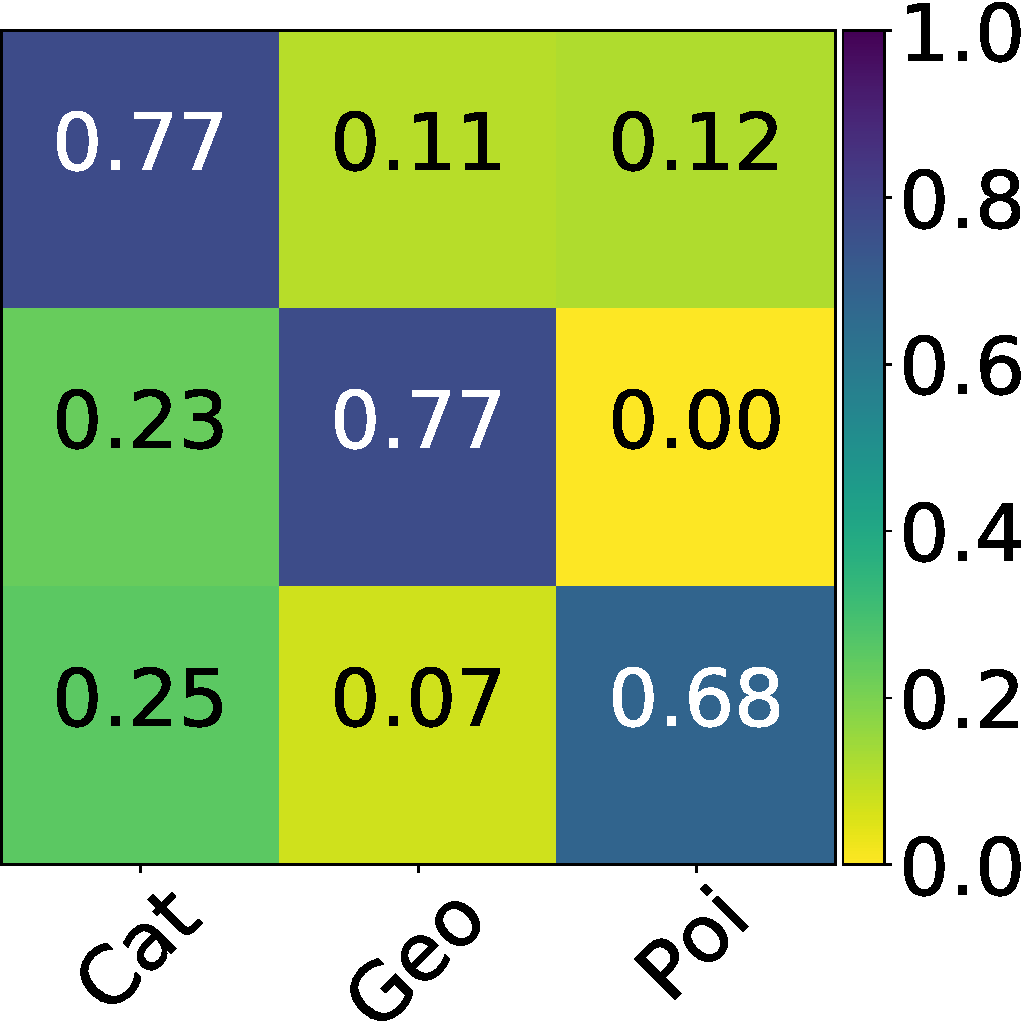
\includegraphics[width=.5\linewidth]{figures/N-10000-disc-param-conf-mat-crop}
    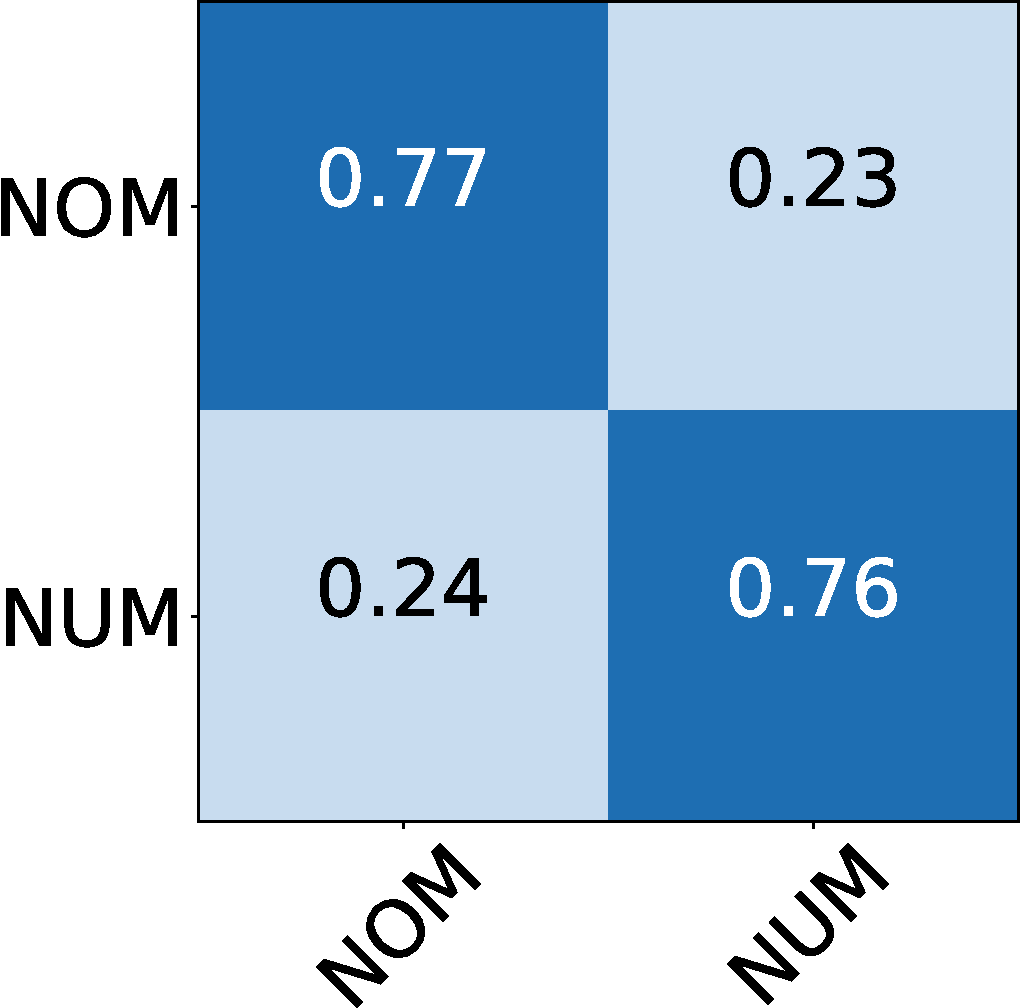
\includegraphics[width=.5\linewidth]{figures/disc-type-conf-mat-crop}\\
  \end{minipage}\hfill\begin{minipage}[t]{0.3\linewidth}
    \vspace{-150pt}
    Uncertainty over likelihood models recovered when a ground truth is available
    
  \end{minipage}\hfill\begin{minipage}[t]{0.3\linewidth}
    \vspace{-150pt}
    
  \end{minipage}
  
\end{frame}

\begin{frame}[t, htt=bgrey2]
  \frametitle{Type inference}

  \large
  \begin{minipage}[t]{0.9\linewidth}
    %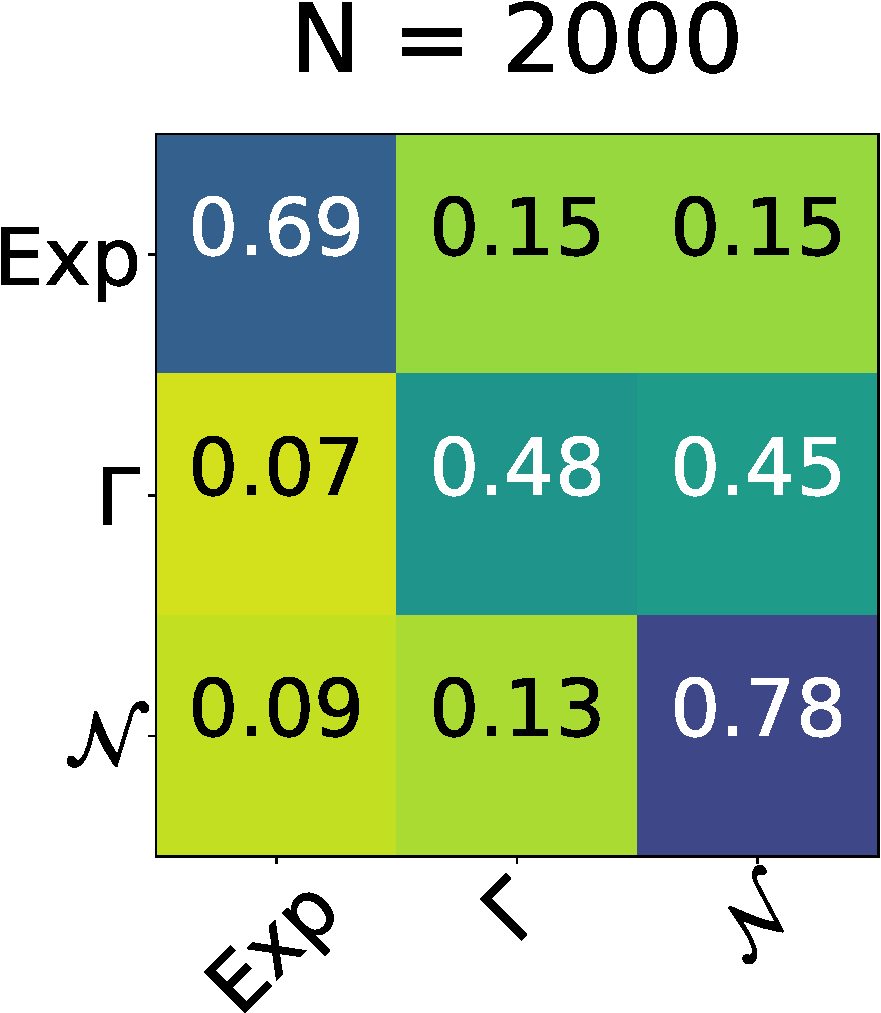
\includegraphics[width=.5\linewidth]{figures/N-2000-cont-param-conf-mat-crop}
    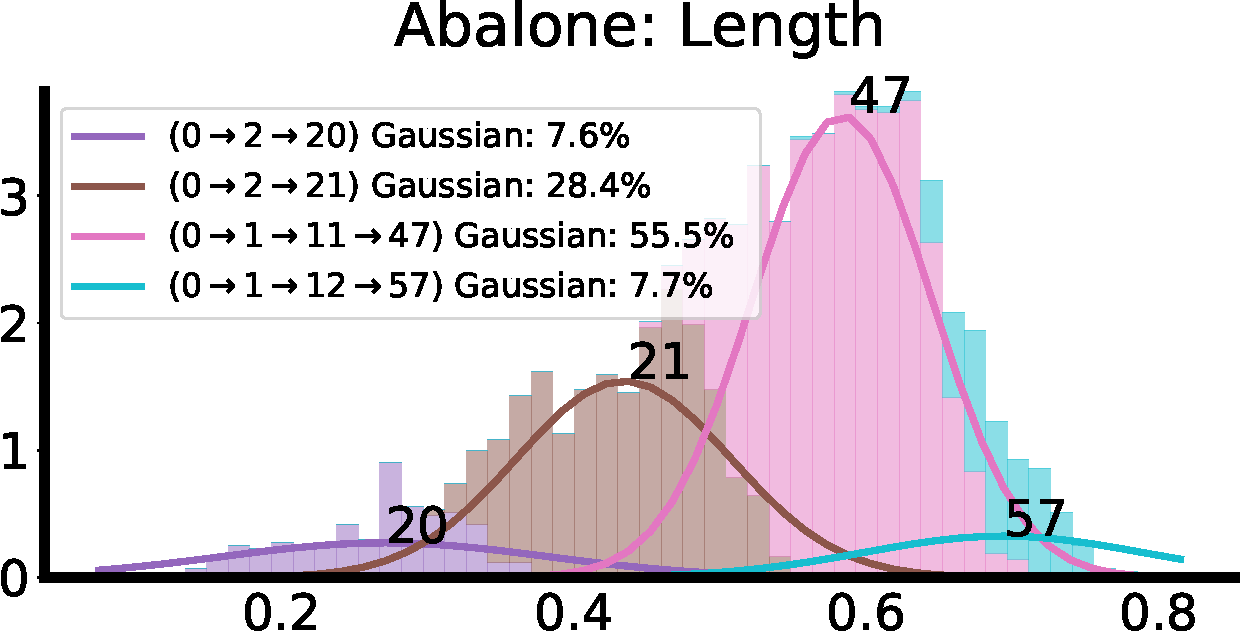
\includegraphics[width=0.45\columnwidth]{figures/d1-fit-crop.pdf}
    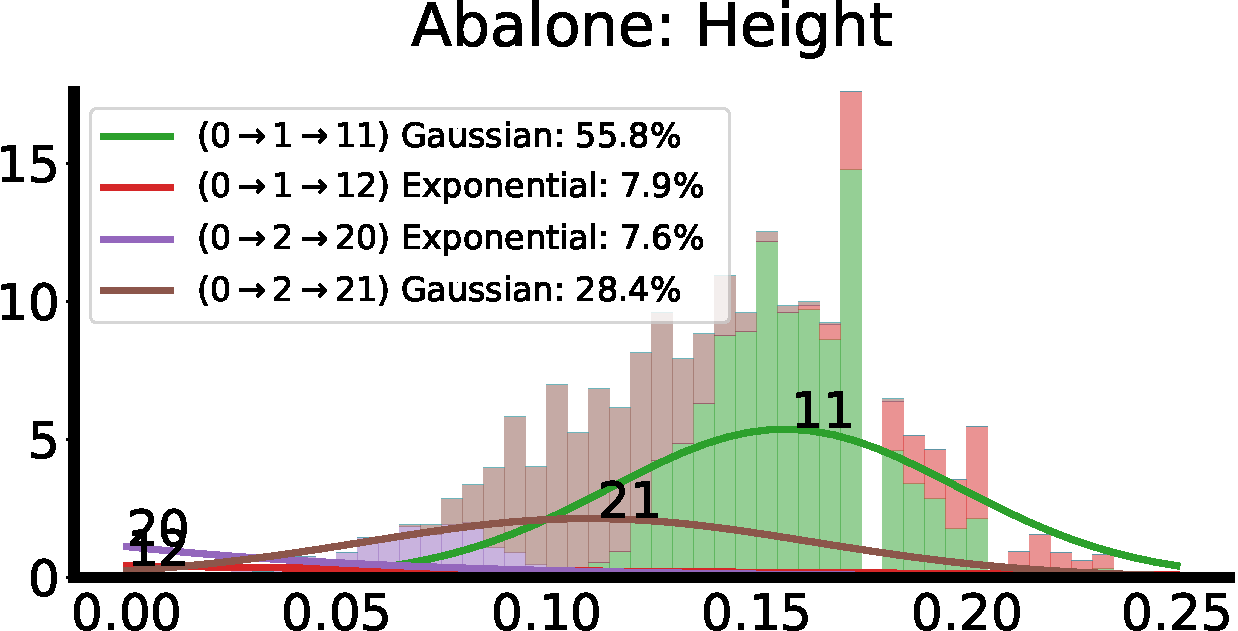
\includegraphics[width=0.45\columnwidth]{figures/d3-fit-crop.pdf}\\
    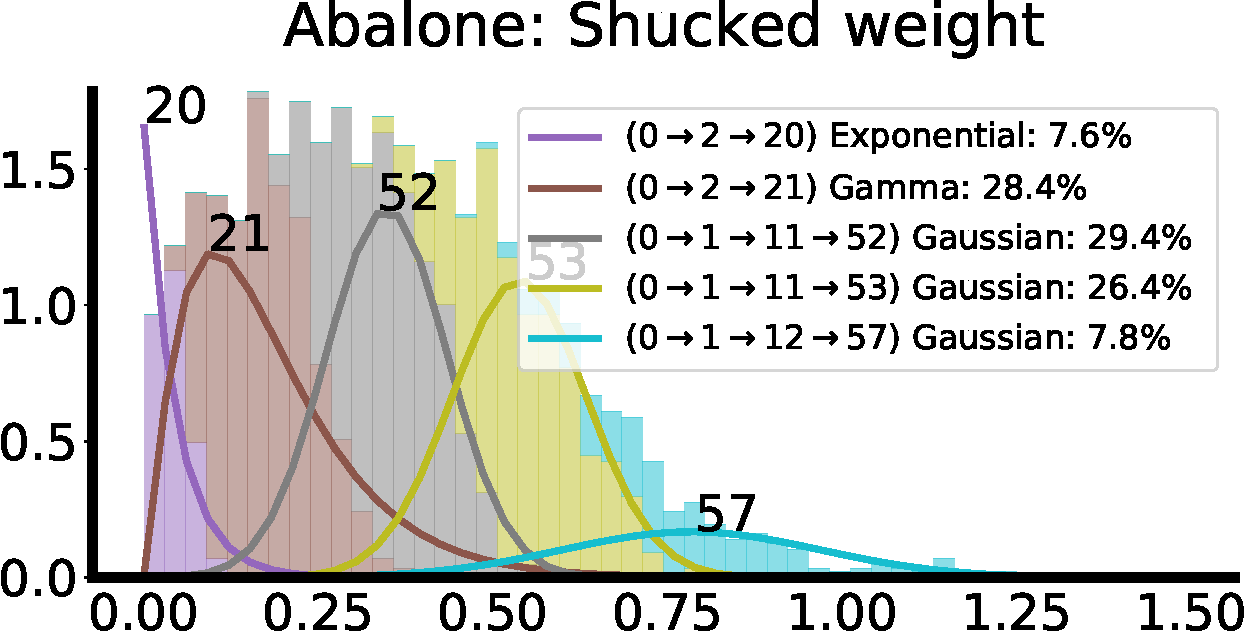
\includegraphics[width=0.45\columnwidth]{figures/d5-fit-crop.pdf}
    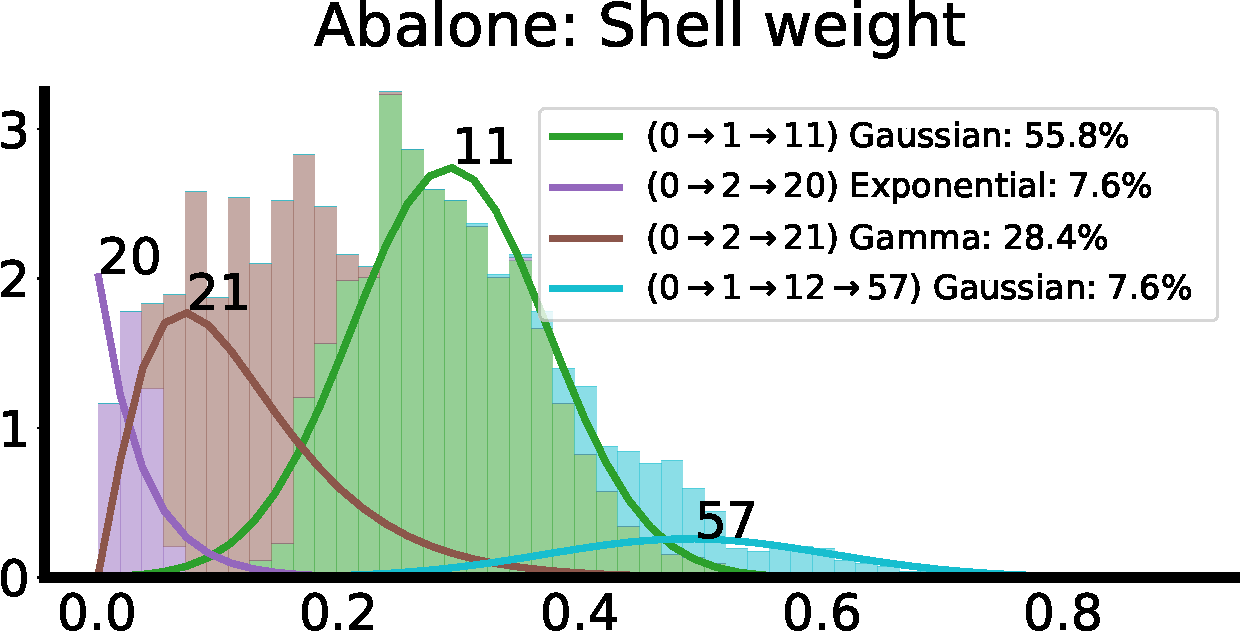
\includegraphics[width=0.45\columnwidth]{figures/d7-fit-crop.pdf}
  \end{minipage}\hfill\begin{minipage}[t]{0.3\linewidth}
    \vspace{-150pt}
    % Uncertainty over likelihood models recovered when a ground truth is available
    
  \end{minipage}\hfill\begin{minipage}[t]{0.3\linewidth}
    \vspace{-150pt}
    
  \end{minipage}
  
\end{frame}

\begin{frame}[t, htt=bgrey2]
  \frametitle{Missing values estimation}

  \large
  \begin{minipage}[t]{0.66\linewidth}
    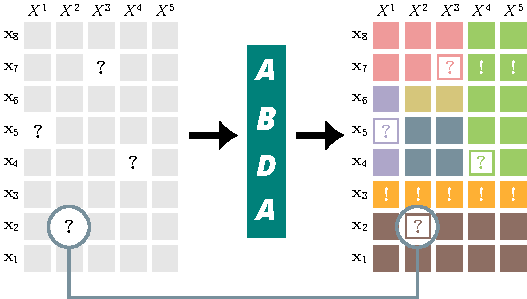
\includegraphics[width=.99\linewidth]{figures/abda-miss}
  \end{minipage}\hfill\begin{minipage}[t]{0.3\linewidth}
    \vspace{-150pt}
    Marginalizing over missing values is easy!\\
    \comment{via SPN inference}\\

    Imputation via MPE inference\\
    $$\tilde{\x}_{n}^{m}=\argmax_{\x_{n}^{m}}\SPN(\x_{n}^{m} \cndbar \x_{n}^{o})$$
    
  \end{minipage}  
\end{frame}

\begin{frame}[t, htt=bgrey2]
  \frametitle{Missing values estimation}

  \large
  \begin{minipage}[t]{0.66\linewidth}
     % \vspace{-35pt}
      \fontsize{17}{18}\selectfont
%       \begin{table}[!t]

% \tiny
%     \setlength{\columnsep}{-10pt}
%     %\centering
%     \begin{tabular}{r r r r r r r r r}
%     % &\multicolumn{6}{c}{\textit{transductive setting}}&\multicolumn{2}{c}{\textit{inductive setting}}\\
%     % \cmidrule(lr{1em}){2-7}\cmidrule(lr{1em}){8-9}
%     &\multicolumn{3}{c}{10\% missing}&\multicolumn{3}{c}{50\%
%                                        missing}\\%&\multicolumn{2}{c}{20\%                                                 test}\\%&\multicolumn{3}{c}{10\%}&\multicolumn{3}{c}{50\%}\\
%     \cmidrule(lr{1em}){2-4}\cmidrule(lr{1em}){5-7}%\cmidrule(lr{1em}){8-9}
%     &\textbf{ISLV}&\textbf{ABDA}&\textbf{MSPN}&\textbf{ISLV}&\textbf{ABDA}&\textbf{MSPN}\\%&\textbf{ABDA}&\textbf{MSPN}\\%&\textbf{ISLV}&\textbf{HSPN}&\textbf{MSPN}&\textbf{ISLV}&\textbf{HSPN}&\textbf{MSPN}\\
%          \textsf{Abalone} & -1.15$\scriptstyle\scriptstyle\pm 0.12$ & -0.02$\scriptstyle\pm0.03$& \textbf{0.20}& -0.89$\scriptstyle\pm 0.36$& -0.05$\scriptstyle\pm0.02$& \textbf{0.14}\\%& 2.22$\scriptstyle\pm0.02$& \textbf{9.73} \\
%          \textsf{Adult} & - & \textbf{-0.60}$\scriptstyle\pm\mathbf{0.02}$ & -3.46& -& \textbf{-0.69}$\scriptstyle\pm\mathbf{0.01}$&  -5.83\\%& \textbf{-5.91}$\scriptstyle\pm\mathbf{0.01}$&-44.07\\
%          %\textsf{Anneal} & - &  & -4.48& & & -4.45& &\\
%          \textsf{Austral.} & -7.92$\scriptstyle\pm0.96$ & \textbf{-1.74}$\scriptstyle\pm\mathbf{0.19}$&  -3.85& -9.37$\scriptstyle\pm0.69$& \textbf{-1.63}$\scriptstyle\pm\mathbf{0.04}$&-3.76\\%& \textbf{-16.44}$\scriptstyle\pm\mathbf{0.04}$&-36.14\\
%          \textsf{Autism} & -2.22$\scriptstyle\pm0.06$ &  \textbf{-1.23}$\scriptstyle\pm\mathbf{0.02}$& -1.54& -2.67$\scriptstyle\pm0.16$& \textbf{-1.24}$\scriptstyle\pm\mathbf{0.01}$& -1.57\\%& \textbf{-27.93}$\scriptstyle\pm\mathbf{0.02}$&-39.20\\
%          \textsf{Breast} & -3.84$\scriptstyle\pm0.05$ &  -2.78$\scriptstyle\pm0.07$& \textbf{-2.69}& -4.29$\scriptstyle\pm0.17$&\textbf{-2.85}$\scriptstyle\pm\mathbf{0.01}$& -3.06\\%&  \textbf{-25.48}$\scriptstyle\pm\mathbf{0.05}$&-28.01\\
%          \textsf{Chess} & -2.49$\scriptstyle\pm0.04$ &\textbf{-1.87}$\scriptstyle\pm\mathbf{0.01}$ & -3.94& -2.58$\scriptstyle\pm0.04$&\textbf{-1.87}$\scriptstyle\pm\mathbf{0.01}$ & -3.92\\%&\textbf{-12.30}$\scriptstyle\pm\mathbf{0.00}$&-13.01\\
%          \textsf{Crx} & -12.17$\scriptstyle\pm1.41$ &  \textbf{-1.19}$\scriptstyle\pm\mathbf{0.12}$& -3.28& -11.96$\scriptstyle\pm1.01$ & \textbf{-1.20}$\scriptstyle\mathbf\pm\mathbf{0.04}$& -3.51\\%&\textbf{-12.82}$\scriptstyle\pm\mathbf{0.07}$ &-36.26\\
%          \textsf{Derma} &-2.44$\scriptstyle\pm 0.23$& \textbf{-0.96}$\scriptstyle\pm\mathbf{0.02}$& -1.00& -3.57$\scriptstyle\pm 0.32$& \textbf{-0.99}$\scriptstyle\pm\mathbf{0.01}$& -1.01  \\%&\textbf{-24.98}$\scriptstyle\pm\mathbf{0.19}$&-27.71\\
%          \textsf{Diabetes} & -10.53$\scriptstyle\pm1.51$ &  \textbf{-2.21}$\scriptstyle\pm\mathbf{0.09}$& -3.88& -12.52$\scriptstyle\pm0.52$& \textbf{-2.37}$\scriptstyle\pm\mathbf{0.09}$& -4.01\\%&\textbf{-17.48}$\scriptstyle\pm\mathbf{0.05}$ &-31.22\\
%          \textsf{German} & -3.49$\scriptstyle\pm 0.21$ & \textbf{-1.54}$\scriptstyle\pm\mathbf{0.01}$& -1.58 & -4.06$\scriptstyle\pm 0.28$& \textbf{-1.55}$\scriptstyle\pm\mathbf{0.01}$& -1.60\\%&  \textbf{-25.83}$\scriptstyle\pm\mathbf{0.05}$&-26.05\\
%          \textsf{Student} & -2.83$\scriptstyle\pm 0.27$ &\textbf{-1.56}$\scriptstyle\pm\mathbf{0.03}$ & -1.57& -3.80$\scriptstyle\pm 0.29$& \textbf{-1.57}$\scriptstyle\pm\mathbf{0.01}$ & -1.58\\%& \textbf{-28.73}$\scriptstyle\pm\mathbf{0.10}$&-30.18 \\
%          \textsf{Wine} &  -1.19$\scriptstyle\pm 0.02$&-0.90$\scriptstyle\pm 0.02$ & \textbf{-0.13}& -1.34$\scriptstyle\pm 0.01$ & -0.92$\scriptstyle\pm 0.01$& \textbf{-0.41}\\%&-10.12$\scriptstyle\pm0.01$&\textbf{-0.13}\\
%          % \cmidrule(lr{1em}){2-4}\cmidrule(lr{1em}){5-7}\cmidrule(lr{1em}){8-9}
%          % wins & 0 & 9 & 3 & 0 & 10 & 2 & 10 & 2\\
%          % \cmidrule{2-9}
%     \end{tabular}
%       %\vspace{-6pt}
% \end{table}
            \begin{table}[!t]

             \small
    \setlength{\columnsep}{-10pt}
    %\centering
    \begin{tabular}{r r r r r r r r r}
    % &\multicolumn{6}{c}{\textit{transductive setting}}&\multicolumn{2}{c}{\textit{inductive setting}}\\
    % \cmidrule(lr{1em}){2-7}\cmidrule(lr{1em}){8-9}
    &\multicolumn{3}{c}{50\%
                                       missing}\\%&\multicolumn{2}{c}{20\%                                                 test}\\%&\multicolumn{3}{c}{10\%}&\multicolumn{3}{c}{50\%}\\
    \cmidrule(lr{1em}){2-4}%\cmidrule(lr{1em}){8-9}
    &\textbf{ISLV}&\textbf{ABDA}&\textbf{MSPN}\\%&\textbf{ABDA}&\textbf{MSPN}\\%&\textbf{ISLV}&\textbf{HSPN}&\textbf{MSPN}&\textbf{ISLV}&\textbf{HSPN}&\textbf{MSPN}\\
         \textsf{Abalone} &  -0.89$\scriptstyle\pm 0.36$& -0.05$\scriptstyle\pm0.02$& \textbf{0.14}\\%& 2.22$\scriptstyle\pm0.02$& \textbf{9.73} \\
         \textsf{Adult} &  -& \textbf{-0.69}$\scriptstyle\pm\mathbf{0.01}$&  -5.83\\%& \textbf{-5.91}$\scriptstyle\pm\mathbf{0.01}$&-44.07\\
         %\textsf{Anneal} & - &  & -4.48& & & -4.45& &\\
         \textsf{Austral.} &   -9.37$\scriptstyle\pm0.69$& \textbf{-1.63}$\scriptstyle\pm\mathbf{0.04}$&-3.76\\%& \textbf{-16.44}$\scriptstyle\pm\mathbf{0.04}$&-36.14\\
         \textsf{Autism} &   -2.67$\scriptstyle\pm0.16$& \textbf{-1.24}$\scriptstyle\pm\mathbf{0.01}$& -1.57\\%& \textbf{-27.93}$\scriptstyle\pm\mathbf{0.02}$&-39.20\\
         \textsf{Breast} & -4.29$\scriptstyle\pm0.17$&\textbf{-2.85}$\scriptstyle\pm\mathbf{0.01}$& -3.06\\%&  \textbf{-25.48}$\scriptstyle\pm\mathbf{0.05}$&-28.01\\
         \textsf{Chess} &  -2.58$\scriptstyle\pm0.04$&\textbf{-1.87}$\scriptstyle\pm\mathbf{0.01}$ & -3.92\\%&\textbf{-12.30}$\scriptstyle\pm\mathbf{0.00}$&-13.01\\
         \textsf{Crx} &   -11.96$\scriptstyle\pm1.01$ & \textbf{-1.20}$\scriptstyle\mathbf\pm\mathbf{0.04}$& -3.51\\%&\textbf{-12.82}$\scriptstyle\pm\mathbf{0.07}$ &-36.26\\
         \textsf{Derma.} &  -3.57$\scriptstyle\pm 0.32$& \textbf{-0.99}$\scriptstyle\pm\mathbf{0.01}$& -1.01  \\%&\textbf{-24.98}$\scriptstyle\pm\mathbf{0.19}$&-27.71\\
         \textsf{Diabetes} &   -12.52$\scriptstyle\pm0.52$& \textbf{-2.37}$\scriptstyle\pm\mathbf{0.09}$& -4.01\\%&\textbf{-17.48}$\scriptstyle\pm\mathbf{0.05}$ &-31.22\\
         \textsf{German} &   -4.06$\scriptstyle\pm 0.28$& \textbf{-1.55}$\scriptstyle\pm\mathbf{0.01}$& -1.60\\%&  \textbf{-25.83}$\scriptstyle\pm\mathbf{0.05}$&-26.05\\
         \textsf{Student} &   -3.80$\scriptstyle\pm 0.29$& \textbf{-1.57}$\scriptstyle\pm\mathbf{0.01}$ & -1.58\\%& \textbf{-28.73}$\scriptstyle\pm\mathbf{0.10}$&-30.18 \\
         \textsf{Wine} &   -1.34$\scriptstyle\pm 0.01$ & -0.92$\scriptstyle\pm 0.01$& \textbf{-0.41}\\%&-10.12$\scriptstyle\pm0.01$&\textbf{-0.13}\\
         % \cmidrule(lr{1em}){2-4}\cmidrule(lr{1em}){5-7}\cmidrule(lr{1em}){8-9}
         % wins & 0 & 9 & 3 & 0 & 10 & 2 & 10 & 2\\
         % \cmidrule{2-9}
    \end{tabular}
      %\vspace{-6pt}
\end{table}

\end{minipage}\hfill\begin{minipage}[t]{0.3\linewidth}
  11 real-world benchmarks from UCI\\

  Repeated exps for different missing values percentages\\

  ABDA is more accurate than ISLV modeling uncertainty over
  statistical data types\\

  and more robust than MSPNs, employing the same data-agnostic
  structure learning 
  
  \end{minipage}  
\end{frame}


\begin{frame}[t, htt=bgrey2]
  \frametitle{Anomaly detection}

  \large
  \begin{minipage}[t]{0.66\linewidth}
    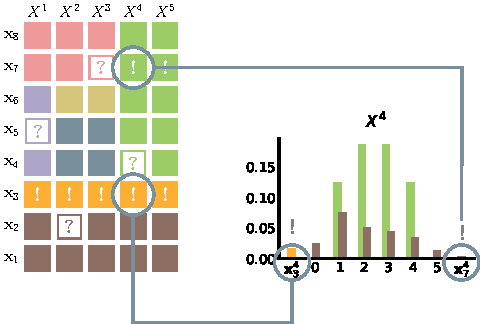
\includegraphics[width=.99\linewidth]{figures/abda-anomaly}
  \end{minipage}\hfill\begin{minipage}[t]{0.3\linewidth}
    \vspace{-150pt}

    ABDA might group outliers into micro-clusters\\

    or relegate them into low-density regions\\
    \comment{tail of distributions}\\
    
     $\log \SPN(\x_{n})$ can be used as a strong signal to indicate
     $\x_{n}$ is an outlier (in the transductive case) or a
     \textit{novelty} (in the inductive case)
     
    
  \end{minipage}  
\end{frame}

\begin{frame}[t, htt=bgrey2]
  \frametitle{Anomaly detection}

  \large
  \begin{minipage}[t]{0.66\linewidth}
    \fontsize{17}{18}\selectfont
  \begin{table}[!t]
%\scriptsize
\small
    \setlength{\tabcolsep}{2pt}
    \begin{tabular}{r r r r r}
    
    %&\multicolumn{4}{c}{outlier detection}\\%&\multicolumn{3}{c}{10\%}&\multicolumn{3}{c}{50\%}\\
    %\cmidrule(l{1em}){1-4}
      \toprule
      &\textsf{1SVM}&\textsf{LOF}&\textsf{HBOS}&\textsf{ABDA}\\%\textsf{MSPN}\\%&\textsf{ISLV}&\textsf{HSPN}&\textsf{MSPN}&\textsf{ISLV}&\textsf{HSPN}&\textsf{MSPN}\\
      \midrule\\
         \textsf{Aloi}&51.71$\scriptstyle\scriptstyle\pm 0.02$&\textbf{74.19}$\scriptstyle\scriptstyle\pm0.70$&52.86$\scriptstyle\scriptstyle\pm
                                          0.53$&47.20$\scriptstyle\scriptstyle\pm 0.02$\\%51.86$\scriptstyle\scriptstyle\pm1.04$&\\
         \textsf{Thyroid}&46.18$\scriptstyle\scriptstyle\pm0.39$&62.38$\scriptstyle\scriptstyle\pm1.04$&62.77$\scriptstyle\scriptstyle\pm3.69$&\textbf{84.88}$\scriptstyle\scriptstyle\pm0.96$\\%77.74$\scriptstyle\scriptstyle\pm0.33$&\\
         \textsf{Breast}&45.77$\scriptstyle\scriptstyle\pm11.1$&98.06$\scriptstyle\scriptstyle\pm0.70$&94.47$\scriptstyle\scriptstyle\pm0.79$&\textbf{98.36}$\scriptstyle\scriptstyle\pm0.07$\\%92.29$\scriptstyle\scriptstyle\pm0.99$&\\
         \textsf{Kdd99}&53.40$\scriptstyle\scriptstyle\pm3.63$&46.39$\scriptstyle\scriptstyle\pm1.95$&87.59$\scriptstyle\scriptstyle\pm4.70$&\textbf{99.79}$\scriptstyle\scriptstyle\pm0.10$\\
         \textsf{Letter}&63.38$\scriptstyle\scriptstyle\pm17.6$&\textbf{86.55}$\scriptstyle\scriptstyle\pm2.23$&60.47$\scriptstyle\scriptstyle\pm1.80$&70.36$\scriptstyle\scriptstyle\pm0.01$\\%68.61$\scriptstyle\scriptstyle\pm0.23$&\\
        \textsf{Pen-glo}&46.86$\scriptstyle\scriptstyle\pm1.02$&87.25$\scriptstyle\scriptstyle\pm1.94$&71.93$\scriptstyle\scriptstyle\pm1.68$&\textbf{89.87}$\scriptstyle\scriptstyle\pm2.87$\\%75.93$\scriptstyle\scriptstyle\pm0.14$&\\
         \textsf{Pen-loc}&44.11$\scriptstyle\scriptstyle\pm6.07$&\textbf{98.72}$\scriptstyle\scriptstyle\pm0.20$&64.30$\scriptstyle\scriptstyle\pm2.70$&90.86$\scriptstyle\scriptstyle\pm0.79$\\%79.25$\scriptstyle\scriptstyle\pm5.41$&\\
         \textsf{Satellite}&52.14$\scriptstyle\scriptstyle\pm3.08$&83.51$\scriptstyle\scriptstyle\pm11.98$&90.92$\scriptstyle\scriptstyle\pm0.16$&\textbf{94.55}$\scriptstyle\scriptstyle\pm0.68$\\%\textbf{95.22}$\scriptstyle\scriptstyle\pm0.45$&\\
         \textsf{Shuttle}&89.37$\scriptstyle\scriptstyle\pm5.13$&66.29$\scriptstyle\scriptstyle\pm1.69$&\textbf{98.47}$\scriptstyle\scriptstyle\pm0.24$&78.61$\scriptstyle\scriptstyle\pm0.02$\\%94.96$\scriptstyle\scriptstyle\pm2.13$&\\
         \textsf{Speech}&45.61$\scriptstyle\scriptstyle\pm3.64$&\textbf{49.37}$\scriptstyle\scriptstyle\pm0.87$&47.47$\scriptstyle\scriptstyle\pm0.10$&46.96$\scriptstyle\scriptstyle\pm0.01$\\%48.24$\scriptstyle\scriptstyle\pm0.67$&\\
          \bottomrule
        %  wins & 0 & 9 & 3 & 0 & 10 & 2 & 10 & 2\\
        %  \cmidrule{2-9}
    \end{tabular}
      %
  \end{table}
  \end{minipage}\hfill\begin{minipage}[t]{0.3\linewidth}
    \vspace{-50pt}

    10 unsupervised outlier detection benchmarks\\

    AUC roc performances\\

    ABDA is competitive vs baselines:\\
    one-class SVMs\\
    Local outlier factor (LOF)\\
    Histogram-based outlier score (HBOS)\\
    ISLV\\
    MSPNs\\
  \end{minipage}  
\end{frame}


\begin{frame}[t, htt=bgrey2]
  \frametitle{Pattern mining}

  \large
  \begin{minipage}[t]{0.66\linewidth}
    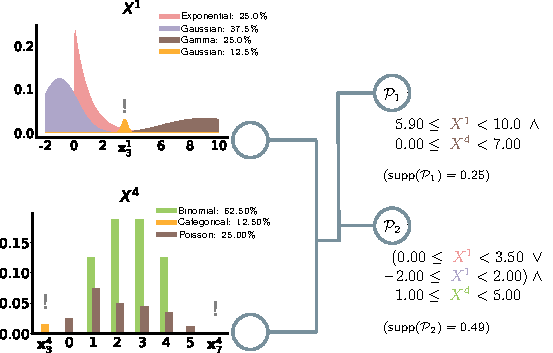
\includegraphics[width=.99\linewidth]{figures/abda-pattern-mining}
  \end{minipage}\hfill\begin{minipage}[t]{0.3\linewidth}
    \vspace{-150pt}

    Extracting a single pattern from each leaf:

    $$\mathcal{P}\colon \pi_{l}^{d}\leq X^{d}<\pi_{h}^{d}$$

    for a certain user-specified thresholding:

    $$\theta: p_{\Leaf^d_{j}}(\mathcal{P}) \geq \theta$$

    Conjunction of patterns can be extracted by looking at partitions
    $\mathcal{P}^{\Node}=\mathcal{P}_{1}\wedge\ldots\wedge\mathcal{P}_{|\scope(\Node)|}$

     
    
  \end{minipage}  
\end{frame}


\begin{frame}[t, htt=bgrey2]
  \frametitle{Pattern mining}

  \large
  \begin{minipage}[t]{0.66\linewidth}
    {\scriptsize\begin{align*}
    %\mathcal{P}_{1}:& 0.0095\leq {\color{red}\mathsf{Height}}< 0.55 (supp(\mathcal{P}_{1})=0.97)\\
    \mathcal{P}_{1}:\quad 0.088&\leq {\color{abagreen}\mathsf{Height}}< 0.224\quad\wedge\\ 
    0.158&\leq {\color{abagreen}\mathsf{ShellWeight}}< 0.425 \quad(supp(\mathcal{P}_{1})=0.507)\\
    \mathcal{P}_{2}:\quad 0.483&\leq {\color{abapink}\mathsf{Length}}< 0.684\quad\wedge\\ 
    0.364&\leq {\color{abapink}\mathsf{Diameter}}< 0.547 \quad(supp(\mathcal{P}_{2})=0.489)\\
    \mathcal{P}_{3}:\quad 0.596&\leq {\color{abagray}\mathsf{WholeWeight}}< 1.040\quad\wedge\\ 
    0.205&\leq {\color{abagray}\mathsf{ShuckedWeight}}< 0.491 \quad\wedge\\
    0.076&\leq {\color{abagray}\mathsf{VisceraWeight}}< 0.281 \quad(supp(\mathcal{P}_{3})=0.223)\\
    \mathcal{P}_{4}:\quad 0.596&\leq {\color{abayellow}\mathsf{WholeWeight}}< 1.040\quad\wedge\\ 
    0.205&\leq {\color{abayellow}\mathsf{ShuckedWeight}}< 0.491 \quad\wedge\\
    0.076&\leq {\color{abayellow}\mathsf{VisceraWeight}}< 0.281 \quad(supp(\mathcal{P}_{4})=0.202)\\
    \mathcal{P}_{5}:\quad 0.313&\leq {\color{ababrown}\mathsf{Length}}< 0.554\quad\wedge\\ 
    \quad 0.230&\leq {\color{ababrown}\mathsf{Diameter}}< 0.438\quad\wedge\\ 
    \quad 0.023&\leq {\color{ababrown}\mathsf{Height}}< 0.197\quad\wedge\\ 
    \quad 0.165&\leq {\color{ababrown}\mathsf{WholeWeight}}< 0.639\quad\wedge\\ 
    0.037&\leq {\color{ababrown}\mathsf{ShuckedWeight}}< 0.408 \quad\wedge\\
    0.019&\leq {\color{ababrown}\mathsf{VisceraWeight}}<0.192 \quad\wedge\\
    0.027&\leq {\color{ababrown}\mathsf{ShellWeight}}< 0.27 \quad\wedge\\
    \quad 5&\leq {\color{ababrown}\mathsf{Rings}}<13\quad(supp(\mathcal{P}_{5})=0.111)\\
\end{align*}
}  
  \end{minipage}\hfill\begin{minipage}[t]{0.3\linewidth}
    \vspace{-50pt}
They can be ranked by their \emph{relevance} or \emph{support}, that
is $p_{\SPN}(\mathcal{P}^{\Node})$.
     
    
  \end{minipage}  
\end{frame}

\begin{frame}[t, htt=mpigreen]
  \frametitle{Automatic exploratory data analysis for non-statisticians}

  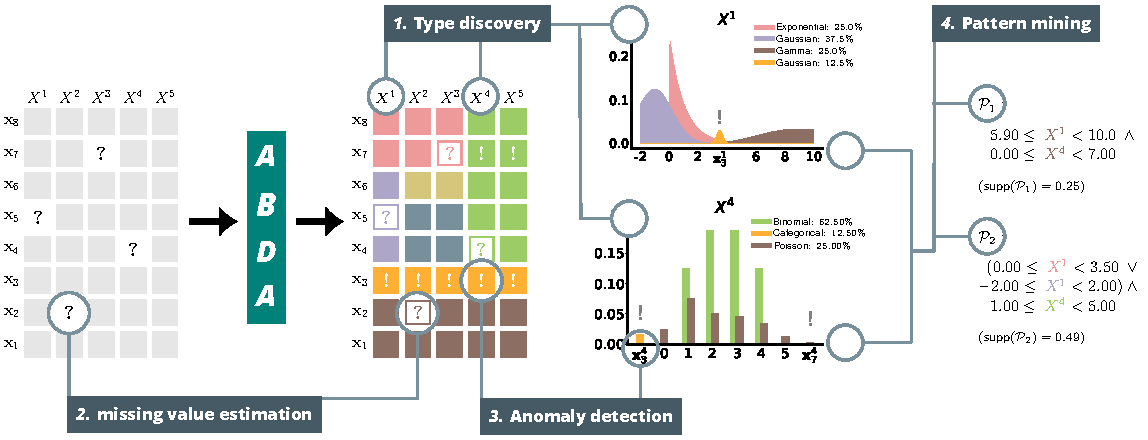
\includegraphics[width=1.04\linewidth]{figures/abda-full}\\

  with ABDA we automate exploratory data analysis and make it
  accessible for non-statisticians!
  
\end{frame}



 
\begin{frame}[allowframebreaks]
  \frametitle{References}
  \setlength\bibitemsep{8pt}
  \printbibliography
\end{frame}

out
\end{document}

%%% Local Variables:
%%% mode: latex
%%% TeX-engine: xetex
%%% TeX-master: t
%%% End:



